\documentclass{article}
\usepackage{tikz}
\usepackage{amsmath}

\begin{document}

\begin{figure}
\centering
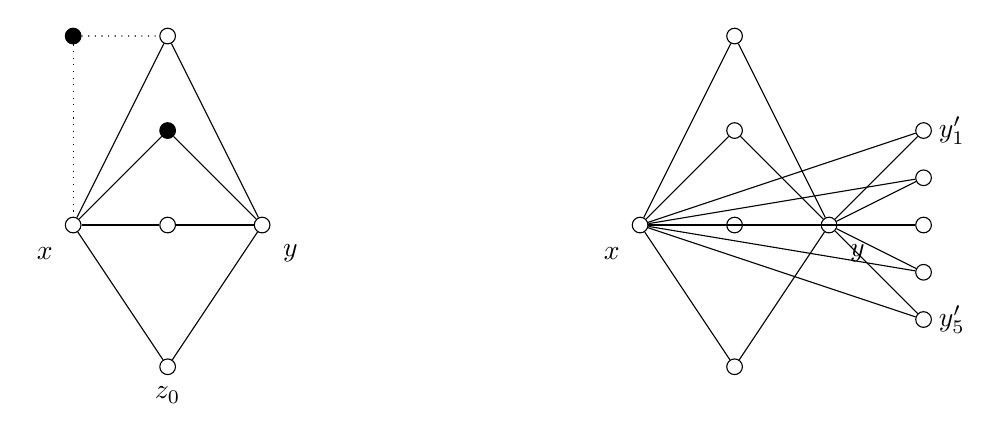
\begin{tikzpicture}[scale=1.2]
% Left diagram
\begin{scope}
    % Vertices
    \node[circle, draw, fill=white, inner sep=2pt] (x) at (0,0) {};
    \node[circle, draw, fill=white, inner sep=2pt] (y) at (2,0) {};
    \node[circle, draw, fill=white, inner sep=2pt] (z0) at (1,-1.5) {};
    \node[circle, draw, fill=white, inner sep=2pt] (z1) at (1,0) {};
    \node[circle, draw, fill=black, inner sep=2pt] (z2) at (1,1) {};
    \node[circle, draw, fill=white, inner sep=2pt] (z3) at (1,2) {};
    \node[circle, draw, fill=black, inner sep=2pt] (w) at (0,2) {};
    
    % Labels
    \node at (-0.3,-0.3) {$x$};
    \node at (2.3,-0.3) {$y$};
    \node at (1,-1.8) {$z_0$};
    
    % Edges
    \draw (x) -- (z0);
    \draw (x) -- (z1);
    \draw (x) -- (z2);
    \draw (x) -- (z3);
    \draw (y) -- (z0);
    \draw (y) -- (z1);
    \draw (y) -- (z2);
    \draw (y) -- (z3);
    
    % Dotted lines
    \draw[dotted] (w) -- (x);
    \draw[dotted] (w) -- (z3);
\end{scope}

% Right diagram
\begin{scope}[xshift=6cm]
    % Vertices
    \node[circle, draw, fill=white, inner sep=2pt] (x) at (0,0) {};
    \node[circle, draw, fill=white, inner sep=2pt] (y) at (2,0) {};
    \node[circle, draw, fill=white, inner sep=2pt] (z0) at (1,-1.5) {};
    \node[circle, draw, fill=white, inner sep=2pt] (z1) at (1,0) {};
    \node[circle, draw, fill=white, inner sep=2pt] (z2) at (1,1) {};
    \node[circle, draw, fill=white, inner sep=2pt] (z3) at (1,2) {};
    \node[circle, draw, fill=white, inner sep=2pt] (y1) at (3,1) {};
    \node[circle, draw, fill=white, inner sep=2pt] (y2) at (3,0.5) {};
    \node[circle, draw, fill=white, inner sep=2pt] (y3) at (3,0) {};
    \node[circle, draw, fill=white, inner sep=2pt] (y4) at (3,-0.5) {};
    \node[circle, draw, fill=white, inner sep=2pt] (y5) at (3,-1) {};
    
    % Labels
    \node at (-0.3,-0.3) {$x$};
    \node at (2.3,-0.3) {$y$};
    \node at (3.3,1) {$y'_1$};
    \node at (3.3,-1) {$y'_5$};
    
    % Edges
    \draw (x) -- (z0);
    \draw (x) -- (z1);
    \draw (x) -- (z2);
    \draw (x) -- (z3);
    \draw (x) -- (y1);
    \draw (x) -- (y2);
    \draw (x) -- (y3);
    \draw (x) -- (y4);
    \draw (x) -- (y5);
    \draw (y) -- (z0);
    \draw (y) -- (z1);
    \draw (y) -- (z2);
    \draw (y) -- (z3);
    \draw (y) -- (y1);
    \draw (y) -- (y2);
    \draw (y) -- (y3);
    \draw (y) -- (y4);
    \draw (y) -- (y5);
\end{scope}
\end{tikzpicture}
\caption{Left: The case $S\nsubseteq N[x]\cup N[y]$ and $|Z|\ge 5$ in the proof of the second statement in Claim~\ref{clm2}. Right: The proof of Claim~\ref{clm3}, where we suppose, to the contrary, that there exists $x_i$ such that $|N(x_i)\cap Y|\ge 5$.}
\end{figure}

\end{document}